\chapter{Experiment}
Our initialization for table assignment was chosen such at each customer is at a separate table at the beginning. Louvain method \cite{blondel2008fast} was used in MCLA algorithm due to its low time complexity.
\section{Synthetic Networks}

\subsection{Setup}

In this section, the performance of proposed method is demonstrated using synthetic network as described below:

\begin{algorithm}[H]
\label{alg:powerlaw}
\caption{Power-Law clustering generator}
\textbf{Input:}\\
    $\gamma$: gamma constant \\
    $K$: number of clusters\\

\textbf{Output:}\\
    $size$: relative sizes of clusters distributed according to density $f(x) \propto x^{-\gamma}$\\
    
\begin{algorithmic}

\State $size = \{\frac{k - 0.5}{K}\}_{k=1}^{K}$

\State $size = size^\frac{1}{1 - \gamma}$ \Comment{Element-wise operation}

\State $size = \frac{size}{size.sum()}$ \Comment{Element-wise operation}

\end{algorithmic}
\end{algorithm}

Stochastic Block Model is used to generate the networks with power-law cluster sizes, average degree and intra-cluster edge probability over inter-cluster edge probability $p_{in} / p_{out} = 10$.

We performed grid search over the set of parameters as follow: Number of vertices $|V| \in \{500, 1000, 1500, 2000\}$, average degree $avgdeg \in \{10, 20, 30, 40, 50\}$, scale parameter $s \in \{1000, 2000, ..., 29000\}$

The same node embedding from \emph{Deepwalk} was used for different scale parameter. We fixed these parameters: $\gamma = 2.5$, embedding dimension $d=50$, walks per vertex $\gamma = 2|E|/|V|$, context size $c = 5$, walk length $l = 3c$, receptive field hop $h=1$, \emph{Deepwalk} epochs = 10 and \emph{ddCRP} epochs = 10 for each run. We took only the last 5 iterations from \emph{ddCRP} as the set of stable states.

We compared two versions: initialized Kmeans using ddCRP and MCLA \textbf{ddcrp-mcla} and initialized Kmeans "k-means++" \textbf{kmeans++} with 10 times of initialization which is builtin within sklearn library.

\subsection{Results}
\subsubsection{Modularity}

\begin{figure}
    \centering
    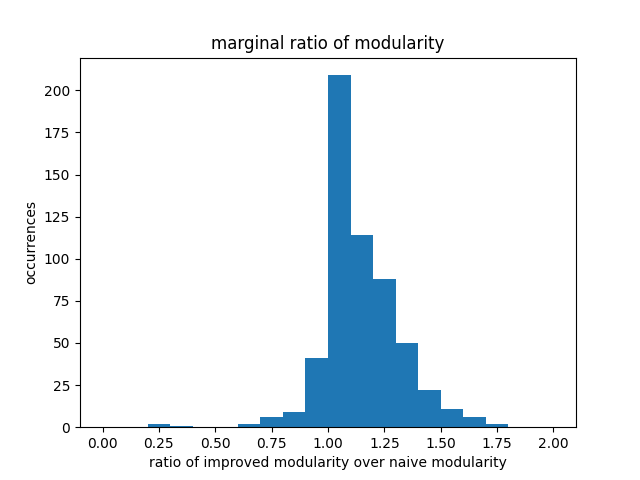
\includegraphics[width=0.8\textwidth]{report/assets/results/ratio.png}
    \caption{Distribution of ratio $\frac{\text{modularity(ddcrp-mcla)}}{\text{modularity(kmeans++)}}$}
    \label{fig:ratio}
\end{figure}


Modularity of each algorithm was evaluated for each setup. Figure \ref{fig:ratio} represent the distribution of the ratio $\frac{\text{modularity(ddcrp-mcla)}}{\text{modularity(kmeans++)}}$. The figure reflects the superior performance of \textbf{ddcrp-mcla} initialization for kmeans as compare to \textbf{kmeans++}. On average, \textbf{ddcrp-mcla} performs better than \textbf{kmeans++} by 14.1\% with a standard deviation of 17.5\%.

Figure \ref{fig:modularity10}, \ref{fig:modularity20}, \ref{fig:modularity30}, \ref{fig:modularity40}, and \ref{fig:modularity50} show that the modularity obtained by \textbf{ddcrp-mcla} always better than \textbf{kmeans++} on all different predicted number of clusters even if the estimation diverges from the true number of clusters (50).

\begin{figure}
    \centering
    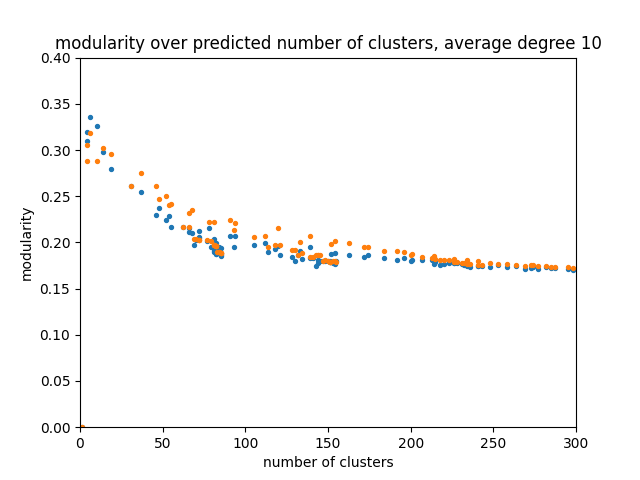
\includegraphics[width=0.8\textwidth]{report/assets/results/modularity10.png}
    \caption{Modularity w.r.t predicted number of clusters for average degree 10 (\textbf{ddcrp-mcla}: orange, \textbf{kmeans++}: blue)}
    \label{fig:modularity10}
\end{figure}

\begin{figure}
    \centering
    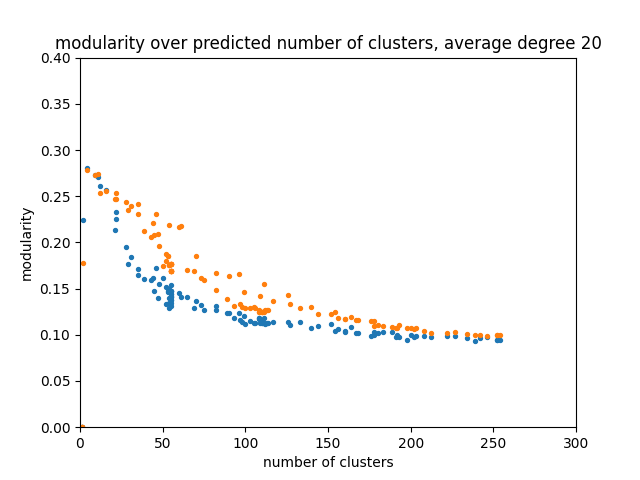
\includegraphics[width=0.8\textwidth]{report/assets/results/modularity20.png}
    \caption{Modularity w.r.t predicted number of clusters for average degree 20 (\textbf{ddcrp-mcla}: orange, \textbf{kmeans++}: blue)}
    \label{fig:modularity20}
\end{figure}

\begin{figure}
    \centering
    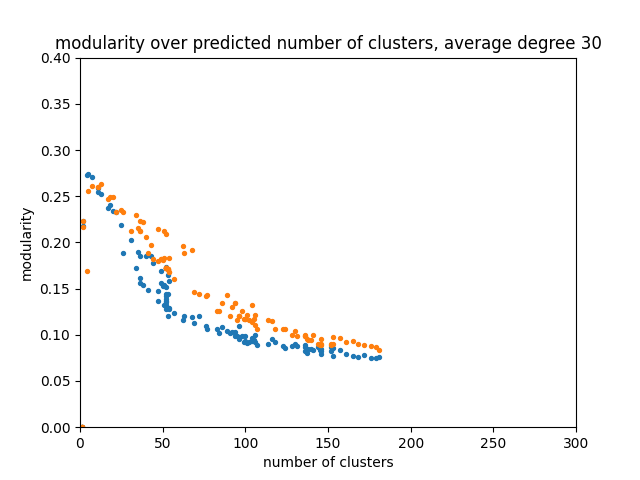
\includegraphics[width=0.8\textwidth]{report/assets/results/modularity30.png}
    \caption{Modularity w.r.t predicted number of clusters for average degree 30 (\textbf{ddcrp-mcla}: orange, \textbf{kmeans++}: blue)}
    \label{fig:modularity30}
\end{figure}

\begin{figure}
    \centering
    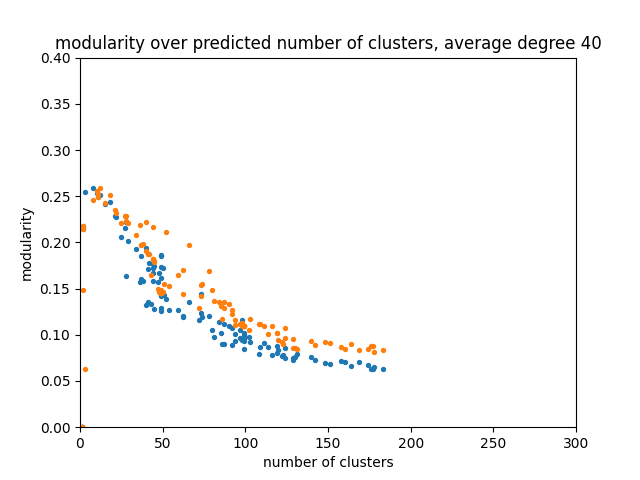
\includegraphics[width=0.8\textwidth]{report/assets/results/modularity40.png}
    \caption{Modularity w.r.t predicted number of clusters for average degree 40 (\textbf{ddcrp-mcla}: orange, \textbf{kmeans++}: blue)}
    \label{fig:modularity40}
\end{figure}

\begin{figure}
    \centering
    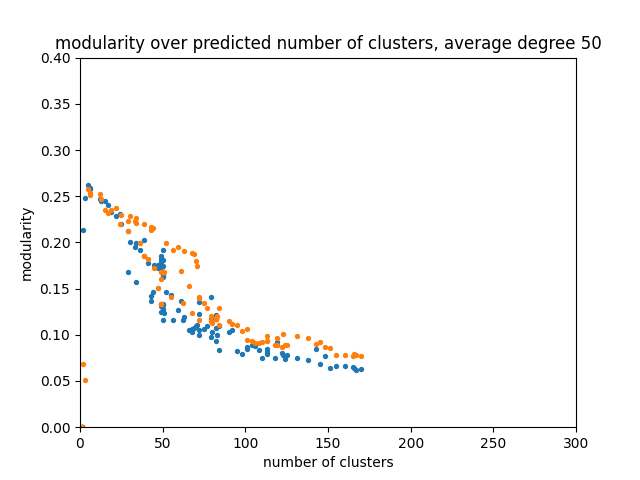
\includegraphics[width=0.8\textwidth]{report/assets/results/modularity50.png}
    \caption{Modularity w.r.t predicted number of clusters for average degree 50 (\textbf{ddcrp-mcla}: orange, \textbf{kmeans++}: blue)}
    \label{fig:modularity50}
\end{figure}

The ratio $\frac{\text{modularity(ddcrp-mcla)}}{\text{modularity(kmeans++)}}$ depends on its predicted number of clusters as shown in figure \ref{fig:ratio_cluster}. The ratio appears to achieve its best performance at the predicted number of clusters between 50 and 100 where the actual number of clusters is 50.

\begin{figure}
    \centering
    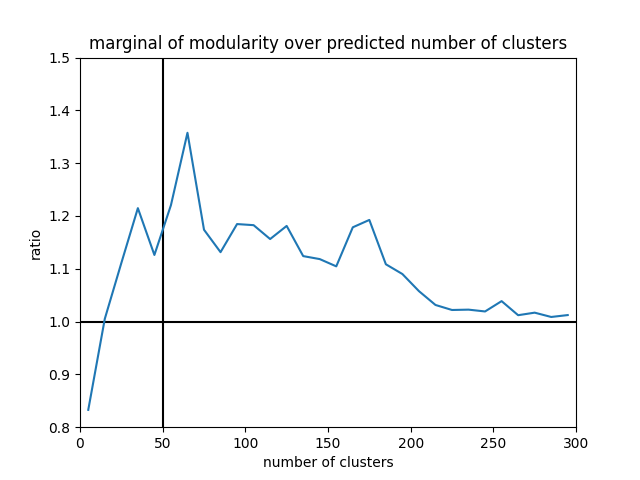
\includegraphics[width=0.8\textwidth]{report/assets/results/ratio_cluster.png}
    \caption{ratio $\frac{\text{modularity(ddcrp-mcla)}}{\text{modularity(kmeans++)}}$ over predicted number of clusters}
    \label{fig:ratio_cluster}
\end{figure}

\section{Real Networks}

\subsection{Setup}

In this experiment, we used the dataset at \cite{paranjape2017motifs}. The temporal network consists of 986 nodes and 332334 temporal edges in the time span of 803 days. We firstly sorted the temporal edges by its timestamp. Then we splitted the set of temporal edges into 1000 equal folds where each fold has roughly 332 edges. We set the window size of 10 folds. After each iteration, we slided the window by 1 fold. We then took the two edge timestamps of the window and filtered all the temporal edges between these timestamps as the set of edges for the graph snapshot.

Similar to the previous experiment, we set embedding dimension $d=50$, walks per vertex $\gamma = 2|E|/|V|$, context size $c = 5$, walk length $l = 3c$, \emph{Deepwalk} epochs = 10 and \emph{ddCRP} epochs = 10 for each run. We took only the last 5 iterations from \emph{ddCRP} as the set of stable states.

We performed grid search over the set of parameters as follow. Receptive field hop $h \in \{1, 2\}$, scale parameter $s \in \{1000, 2000, ..., 8000\}$

\subsection{Results}
\subsubsection{Modularity}
Figure \ref{fig:ratio_cluster_real} shows the ratio between $\frac{\text{modularity(ddcrp-mcla)}}{\text{modularity(kmeans++)}}$ over different predicted number of clusters. If we limit the predicted number of clusters to be greater than 60, the \textbf{ddcrp-mcla} method performs better than \textbf{kmeans++} by 4.4\% with a standard deviation of 5.6\%.

\begin{figure}
    \centering
    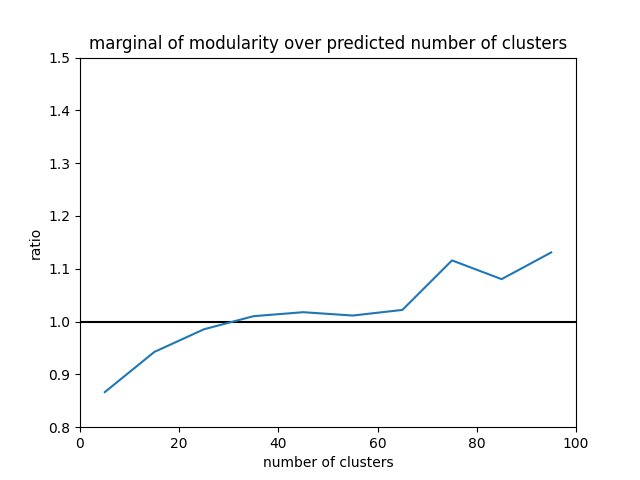
\includegraphics[width=0.8\textwidth]{report/assets/results/ratio_cluster_real.png}
    \caption{ratio $\frac{\text{modularity(ddcrp-mcla)}}{\text{modularity(kmeans++)}}$ over predicted number of clusters}
    \label{fig:ratio_cluster_real}
\end{figure}

\subsubsection{Clustering Evolution}

Our \emph{MCLA} algorithm is capable to produce some useful response from the evolution of clustering. Noted that, these results are completely automated. Textbox \ref{textbox:message}.

\fbox{\begin{minipage}{15em}
message type: join

	9 nodes remained
	
	3 nodes joined
	
	0 nodes left
	
message type: old

	2 nodes remained
	
	0 nodes joined
	
	0 nodes left
	
message type: old

	0 nodes remained
	
	25 nodes joined
	
	7 nodes left
	
message type: old

	3 nodes remained
	
	0 nodes joined
	
	0 nodes left
	
message type: join

	418 nodes remained
	
	0 nodes joined
	
	153 nodes left
	
	...
\label{textbox:message}
\end{minipage}}